% !TEX root = ../EntropicNumeric.tex

\subsection{Unbalanced Barycenters}
\label{sec_appli_bary}

\paragraph{Well-posedness.}
Barycenters and related problems have been defined in Section \ref{subsec_barycenter}. Assume we are given a family of $n$ measures $(p_k \d x )_{k=1}^n$, families of entropies $(\phi_{1,k})_{k=1}^n$ and $(\phi_{2,k})_{k=1}^n$ and families of cost functions $(c_k)_{k=1}^n$. For a clearer picture, let us focus on the case where 
\eq{
 \phi_{2,k}=\alpha_k \cdot \lambda \cdot \varphi \quad \text{for} \quad k=1,\ldots,n
 }
where $\varphi$ is a nonnegative entropy function, $(\alpha_k)_{k=1}^n \in ]0,\infty[^n$ are weights and $\lambda>0$ is a (redundant) parameter. It is also convenient to slightly modify (for this Section only) the definition of the $\KL$ divergence given in \eqref{eq_KLdens} by introducing weights as
\eq{
\KL(r|s) \eqdef \sum_k \alpha_k \cdot \KL(r_k|s_k) \, .
}
No theoretical aspect is affected by this small change, but the definition of the kernel has to be adapted, for each component, as
\eq{
K_k = \exp (-{c_k}/(\alpha_k\, \epsilon))
}
so that one still has $\langle c, r \rangle + \epsilon \KL(r|1) = \epsilon \KL(r|K)+\textnormal{const}$.
%
By equation \eqref{eq_barycenter}, the barycenter problem with entropic regularization corresponds to defining   
\eq{
F_1(r)  = \sum_{k=1}^n \Divergm_{\phi_{k,1}}(r_k \d x| p_k \d x)
\qandq
F_2(s) = \inf_{\sigma\in \Mm_+(Y)} \lambda \sum_{k=1}^n  \alpha_k \Divergm_{ \phi}(s_k \d y| \sigma)
}
(for all $r\in \Lun(X)^n$ and $s\in \Lun(Y)^n$) in \eqref{eq-general-regul-KL}. It is direct to see that the proximal operator of $F_1$ for the $\KL$ divergence (according to our specific definition of $\KL$) can be computed component wise as 
\eql{\label{eq_proxcomponentbary}
\prox^{\KL}_{F_1}(r) = (\prox_{\Diverg_{\phi_{1,1}}(\cdot | p_1)}^{\KL}(r_1),\dots,\prox_{\Diverg_{\phi_{n,1}}(\cdot | p_n)}^{\KL}(r_n)) 
}
so we can use the results from the previous section (recall that $\Diverg$ denotes divergences between functions as in \eqref{eq_divergencefunctions}). Let us turn our attention to the function $F_2$. As it is assumed $\phi(0)\geq0$, $F_2$ is not changed by taking the infimum over $\sigma$ of the form $h \cdot \d y$ for $h\in \Lun(Y)$.
%As a function of $(s_k,h)$ this function has interesting properties. %They are described in the next Lemma, where we also use the notation
%\eq{
%\ol{\Diverg}_\phi : \RR^2 \ni (s,h) \mapsto
%\begin{cases}
%\phi(s/h)h & \text{if $h>0$} \\
%\phi'_\infty \cdot s & \text{otherwise, with $\infty\times0=0$.}
%\end{cases}
%}
%
So one can express $F_2$ for $s\in \Lun(Y)^n$, with notation of \eqref{eq_divergencefunctions} as
\eql{\label{eq_Fbary}
F_2(s) = \min_{h\in \Lun(Y)}  \lambda \sum_{k=1}^n \alpha_k \Diverg_{\phi} (s_k|h) =  \min_{h\in \Lun(Y)}  \lambda \sum_{k=1}^n \alpha_k \int_X \ol{\Diverg}_{\phi} (s_k(x)|h(x)) \d x\, .
}
%
\begin{proposition}
If $\phi'_\infty>0$ then $F_2$ is an admissible integral functional in the sense of Definition \ref{def_integralfunctional} and for all $s\in \Lun(Y)^n$, there exists a minimizer $h\in \Lun(Y)$. 
Moreover, if $r^\star \in \Lun(X\times Y)^n$ minimizes \eqref{eq-general-regul-KL}, then the associated minimizer $h^\star$ is a pointwise minimizer of \eqref{eq_Fbary} at the point $s=P^Y_\# r^\star$.
\end{proposition}
\begin{proof}
Let $G(s,h)$ be the function on the right side, which is an admissible integral functional (see Proposition \ref{prop_divergnormalint} in Appendix \ref{sec:ApxDivergences}). Let us verify the assumptions of the ``reduced minimization Theorem'' \cite[Corollary 3B]{rockafellar1976integral}. Assumption (i) is satisfied because $\phi'_\infty>0$ guarantees the growth condition \cite[2R]{rockafellar1976integral} and assumption (ii) is guaranteed by the fact that if $u\in \Lun(Y)$ and $\Diverg_\phi(u|v)<\infty$ then $v\in \Lun(Y)$ (this is proven by adapting slightly the proof of Lemma \ref{lem_KL_L1}, using the---at least linear--- growth of $\phi$). Thus the cited Corollary applies.
\end{proof}
%
%%%%%%%%%%%%%%%%%%%%%%
%
\paragraph{Derivation of the algorithm.}
According to Proposition \ref{prop_proxKLcont}, computing the $\prox$ and $\proxdiv$ operators requires to solve, for each point $y \in Y$, a problem of the form
\eql{
\label{eq_prox_barycenter}
\min_{(\tilde{s},h)\in \RR^n\times \RR}
\sum_{k=1}^n \alpha_k \left( \epsilon \cdot \ol{\KL} (\tilde{s}_k |s_k) + \lambda \cdot \ol{\Diverg}_\phi (\tilde{s}_k | h) \right)\,.
}
If $\phi$ is smooth, first order optimality conditions for \eqref{eq_prox_barycenter} are simple to obtain. The next Proposition deals with the general case where more care is needed.
%
\begin{proposition}
\label{prop_barycenter_general}
Let $(s_i)_{i=1}^n\in \RR_+^n$. Assume that there exists a feasible candidate $(\tilde{s}^0,h^0)$ for \eqref{eq_prox_barycenter} such that $(s_i>0) \Rightarrow (\tilde{s}^0_i>0)$. A candidate $(\tilde{s},h)$ is a solution of \eqref{eq_prox_barycenter} if and only if 
\begin{itemize}
\item $(s_i=0) \Leftrightarrow (\tilde{s}_i=0)$ and 
\item there exists $b \in\RR^n$ such that $\sum_{k=1}^n \alpha_k b_k =0$ and, for all $k\in \{1,\dots, n\}$, $(a_k,b_k) \in \partial \Diverg_{\phi}(\tilde{s}_k | h)$ with $a_k \eqdef \frac{\epsilon}{\la} \log \frac{s_k}{\tilde{s}_k}$ if $s_k>0$ and $b_k \in \partial_2 \Diverg_\phi(0,h)$ otherwise.
\end{itemize}
\end{proposition}
%
%\todo{Write somewhere a Lemma of positivity (like theorem 2.7 is Borwein Lewis) (related to existence of dual opt)}
\begin{proof}
First assume that $s_i>0$ for all $i\in \{1,\dots ,n\}$. The positivity assumption on the feasible point implies that the sum of the subdifferential is the subdifferential of the sum by continuity of $\KL$ for positive arguments.  Moreover, a minimizer necessarily satisfies $\tilde{s}_i>0$ for all $i$. Consequently, the subderivative of the function in \eqref{eq_prox_barycenter} at $((\tilde{s}_i)_n,h)$ is the set of vectors in $\RR^{n+1}$ of the form
\eq{
\begin{pmatrix}
\vdots \\
\epsilon \alpha_i \log (\tilde{s}_i/s_i) + \lambda \alpha_i a_i  \\
\vdots \\
\lambda \sum_k \alpha_k b_k
\end{pmatrix}
}
with $(a_i,b_i) \in \partial \Diverg_{\phi}(\tilde{s}_i | h)$. Writing the first order optimality condition yields the second condition of the Proposition. Now for all $i$ such that $s_i$ is null, set $\tilde{s}_i=0$ (this is required for feasibility) and do the reasoning above by withdrawing the variables $\tilde{s}_i$ which have been fixed.
\end{proof}
%
Note that once the optimal $h$ is found (possibly with the help of the optimality conditions of Proposition \ref{prop_barycenter_general}), determining the optimal values for $\tilde{s}$ can be done component wise as in \eqref{eq_proxcomponentbary} with the help of Proposition \ref{prop_UOTprox}.
%
In Table \ref{prop_estimatebary} we provide formulas for $h$ for some examples (proofs can be found in Appendix \ref{sec:AppendixBarycenterIterates}), for the subsequent computation of $\tilde{s}_k$ (and the $\proxdiv$ step) we refer the reader to Table \ref{table_proximalexplicit} (where of course one must replace $p$ by $h$).
%
%
%
%
\begin{table}[h] \centering
%\arraystretch
\begin{tabular}{@{}lrcl@{}}\toprule
&$\Diverg_\phi$ && Formula for $h$ as a function of $s\in \RR^n$ \\ \midrule \addlinespace 
(i)&$ \iota_{\{=\}} $
&&$h= \left( \prod_k s_k^{\alpha_k} \right)^{\frac{1}{\sum_k \alpha_k}}$
\\ \addlinespace \addlinespace 
(ii)&$\lambda \KL  $
&&  $h = \left( \frac{\sum_k \alpha_k s_k^{\frac{\epsilon}{\epsilon+\la}} }{\sum_k \alpha_k} \right)^{\frac{\epsilon + \la}{\epsilon}}$
\\ \addlinespace \addlinespace 
(iii)&$\lambda \TV$
&& if $\sum_{k\notin I_+} \alpha_k \geq \sum_{k\in I_+} \alpha_k $ then $h=0$ otherwise solve:\\ \addlinespace
&&& $\sum_{k\notin I_+} \alpha_k+ \sum_{k\in I_+}\alpha_k \max \left( -1 , \min \left( 1 , \frac{\epsilon}{\lambda } \log \frac{h}{s_i}\right) \right) = 0$
\\ \addlinespace \addlinespace
(iv)&$ \RG_{[\beta_1,\beta_2]} $
&&  if $s_k=0$ for some $k$ then $h=0$ otherwise solve:\\ \addlinespace
&&&$\sum_k \alpha_k \left[ \beta_2 \min\left( \log \frac{\beta_2\, h}{s_k} ,0 \right) + \beta_1 \max \left( \log \frac{\beta_1\, h}{s_k} ,0\right) \right] =0$
\\ \addlinespace \addlinespace \bottomrule
\end{tabular}
\caption{Expression for the minimizer $h$ of \eqref{eq_prox_barycenter} as a function of $s\in \RR^n$ where $I_+ = \{k \, ; \, s_k>0 \}$ (proofs in Appendix \ref{sec:AppendixBarycenterIterates}). For the implicit equations of cases (iii) and (iv), an exact solution can be given quickly because computing $\log h$ consists in finding the root of a piecewise linear non-decreasing function (with at most $2n$ pieces), which is guaranteed to change its sign.}
\label{prop_estimatebary}
\end{table}
%
%
%\begin{remark}
%Some comments are in order before the presentation of the numerical experiments:
%\begin{itemize}
%\item For the implicit equations of cases (iii) and (iv), an exact solution can be given quickly because computing $\log h$ consists in finding the root of a piecewise linear non-decreasing function (with at most $2n$ pieces), which is guaranteed to change its sign.
%
%\item Since $\W$ and $\WF$ are geodesic distances (see Sections \ref{subsec_balanced} and \ref{subsec_unbalanced}), computing the barycenter between two measures $\mu$ and $\nu$ with weights $(\theta, 1-\theta)$ amounts to evaluating the geodesic between $\mu$ and $\nu$ at time $\theta$.
%\end{itemize}
%\todo{ B (?) : Add comment about weak convergence of Barycenters? And that finite $\epsilon$ is not so bad and visually more pleasing for this case?}
%\end{remark}
%
%\begin{proposition}
%Let $\Diverg_\phi(x|y)= \iota_{x=y}$ and $(z_i)_n\in [0,\infty[^n$. The unique solution of  \eqref{eq_prox_barycenter} is
%\eq{
%y = \left( \prod_i z_i^{\alpha_i} \right)^{\frac{1}{\sum_i \alpha_i}}
%\qandq
%\frac{x_i}{z_i}  = \frac{y}{z_i}  \, .
%}
%\end{proposition}
%\begin{proposition}
%Let $\phi = \phi_{\KL}$ and $(z_i)_n\in [0,\infty[^n$. The unique solution of  \eqref{eq_prox_barycenter} is
%\eq{
%y = \left( \frac{\sum_i \alpha_i z_i^{\frac{\epsilon}{\epsilon+\la}} }{\sum_i \alpha_i} \right)^{\frac{\epsilon + \la}{\epsilon}}
%\qandq
%\frac{x_i}{z_i}  = \left( \frac{y}{z_i}\right)^{\frac{\la}{\epsilon+\la}} \, .
%}
%\end{proposition}
%
%
%\begin{proposition}
%Let $\phi = \phi_{\TV}$, let $(z_i)_n\in [0,\infty[^n$ and set $I = \{i \, ; \, z_i>0 \}$. All solutions $((x_i)_n,y)$ of \eqref{eq_prox_barycenter} are given by $y=0$ if $\sum_{i\notin I} \alpha_i \geq \sum_{i\in I} \alpha_i $ and $y$ is a solution of
%\eql{
%\label{eq_barycenter_TV}
%\sum_{i\notin I} \alpha_i+ \sum_{i\in I}\alpha_i \max \left( -1 , \min \left( 1 , \frac{\epsilon}{\lambda } \log \frac{y}{z_i}\right) \right) = 0
%}
%otherwise. In all cases, if $z_i\neq0$,
%\eq{
%	\frac{x_i}{z_i} = \min \left( e^{\frac\la\epsilon}, \max \left( e^{-\frac\la\epsilon},\frac{y}{z_i} \right) \right) \, .
%}
%\end{proposition}
%
%Here is how the formula for $y$ should be interpreted: assume all $z_i$ are positive, etc.
%
%Our last example deals with barycenters with a ``range'' constraint.
%\begin{proposition}
%Let $\phi = \iota_{[\beta_1,\beta_2]}$ with $0< \beta_1  \leq \beta_2 < \infty$ and let $(z_i)_n\in [0,\infty[^n$. All solutions $((x_i)_n,y)$ of \eqref{eq_prox_barycenter} are given by $y=0$ if $z_i=0$ for some $i$ and
%\eql{
%\label{eq_barycenter_range}
%\sum_i \alpha_i \left[ \beta_2 \min\left( \log \frac{\beta_2\, y}{z_i} ,0 \right) + \beta_1 \max \left( \log \frac{\beta_1\, y}{z_i} ,0\right) \right] =0
%}
%and, for $z_i>0$, 
%\eq{
%	\frac{x_i}{z_i} = \min \left( \frac{\beta_2 \, y}{z_i}, \max \left( \frac{\beta_1 \, y}{z_i},1 \right) \right)\, .
%}
%\end{proposition}
%
\paragraph{Numerical experiments.}
In Figure \ref{fig_1Dbarycenter}, we display Fr\'echet means-like experiments for a family of $4$ given marginals where $X=Y$ is the segment $[0,1]$ discretized into $I=J=512$ uniform samples with the discretized Lebesgue measure $\mathbf{\d x}$. The (discrete) densities of the marginals $(\mathbf{p}_k)_{k=1}^4$ consist each of the sum of three bumps (centered near the points $x=0.1$, $x=0.5$ and $x=0.9$). These computations where performed with Algorithm \ref{algo_scaling_stabilized} which was stopped after $1500$ iterations (running time of $30$ seconds approximately) and with $\epsilon=10^{-5}$. We observe that relaxing the marginal constraints (Figures \ref{fig_bary1d_KL}-\ref{fig_bary1d_WF}) allows to conserve this structure in three bumps in contrast to classical optimal transport (Figure \ref{fig_bary1d_OT}).

Figure \ref{fig_wasserstein_triangle} and \ref{fig_GHK_triangle} display barycenters for the Wasserstein and the $\GHK$ metric (defined in Section \ref{subsec_unbalanced}) between three densities on $[0,3]^2$ discretized into $200\times 200$ samples. Computations where performed using Algorithm \ref{algo_scaling_discrete} and the ``separable kernel'' method (see Section \ref{sec_implementation}) which was stopped after $1500$ iterations (running time of $70$ seconds approximately) with $\epsilon=9.10^{-4}$. The barycenter coefficients are the following:
\begin{gather*}
(0,1,0)\\
(1,3,0)/4 \qquad (0,3,1)/4 \\
(2,2,0)/4 \qquad (1,2,1)/4 \qquad (0,2,2)/4 \\
(3,1,0)/4 \qquad (2,1,1)/4 \qquad (1,1,2)/4 \qquad (0,1,3)/4\\
(1,0,0)    \qquad (3,0,1)/4 \qquad (2,0,2)/4 \qquad (1,0,3)/4 \qquad (0,0,1)
\end{gather*}
The input densities have a similar global structure: each is made of three distant ``shapes'' of varying mass. The comparison between Figures  \ref{fig_wasserstein_triangle} and \ref{fig_GHK_triangle} lead to a similar remark than for Figure \ref{fig_1Dbarycenter}: relaxing the strict marginal constraints allows to maintain the global ``structure'' of the input densities.

%%%%%%%%%%%%%%%%%%%%%%%%%%%%%%%%%%%%%%%%%%
\begin{figure}
 \centering
 %
\begin{subfigure}{0.5\linewidth} 
\centering
 \resizebox{1.\linewidth}{!}{
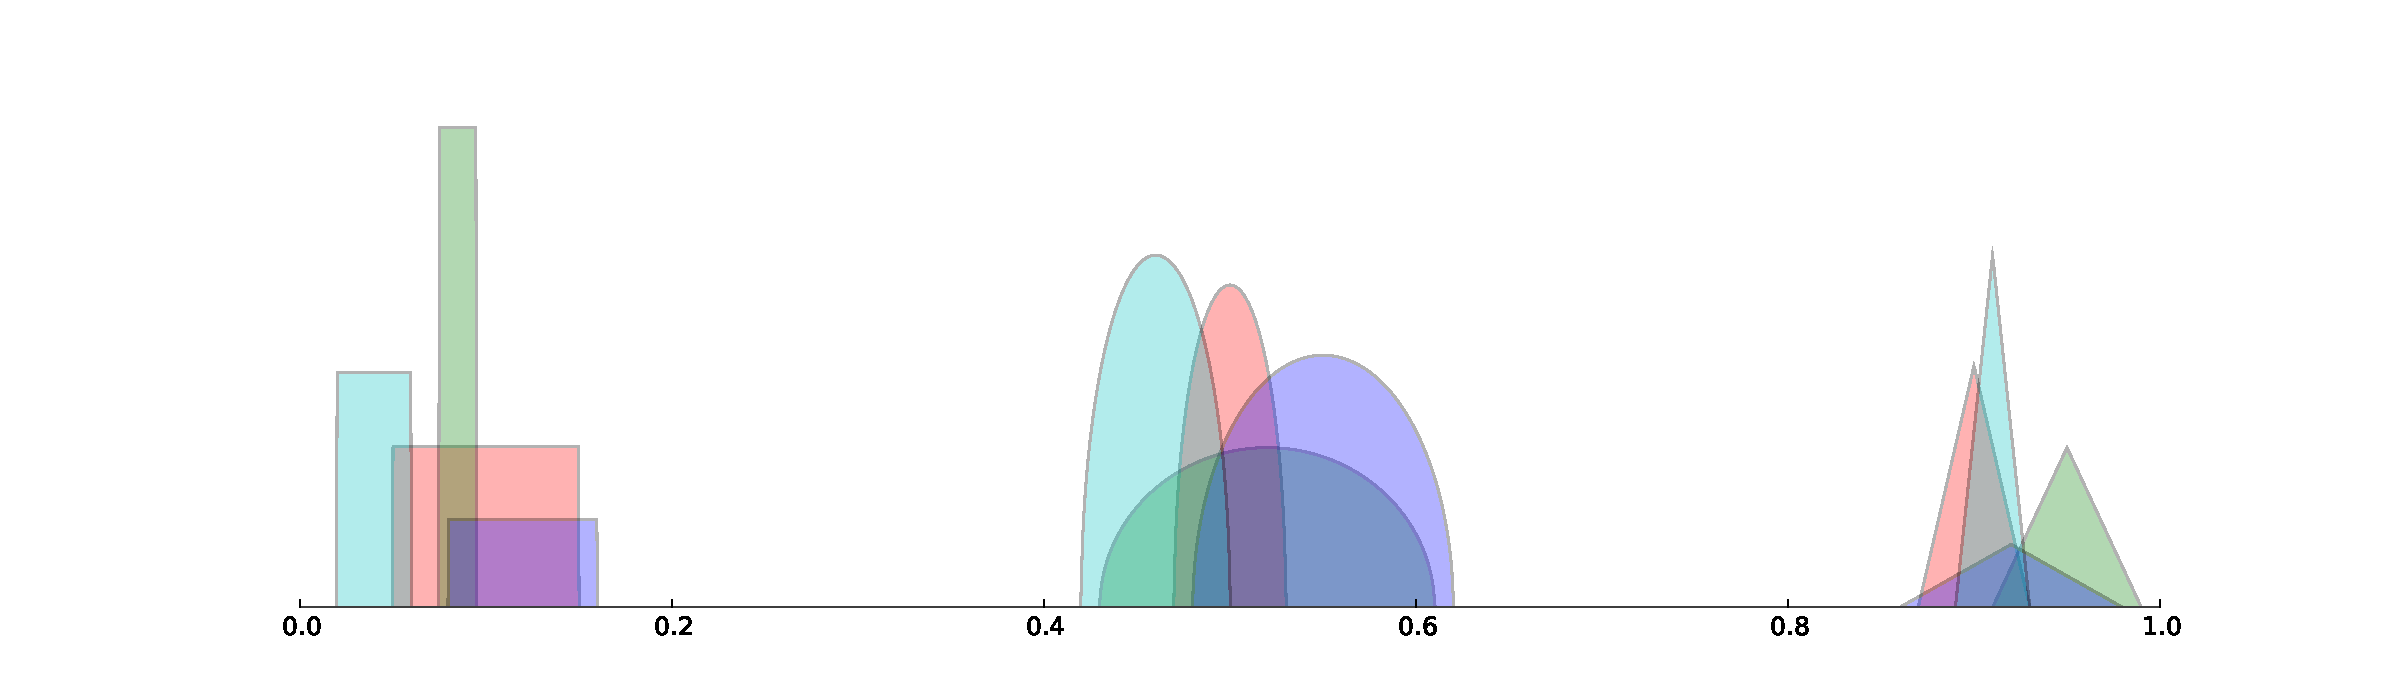
\includegraphics[clip,trim=0cm 0cm 0cm 0cm]{images/barycenter1d/barycenter1d_margs}
}
\caption{Marginals $(\mathbf{p}_k)^4_{k=1}$}
\end{subfigure}%
\begin{subfigure}{0.5\linewidth} 
\centering
 \resizebox{1.\linewidth}{!}{
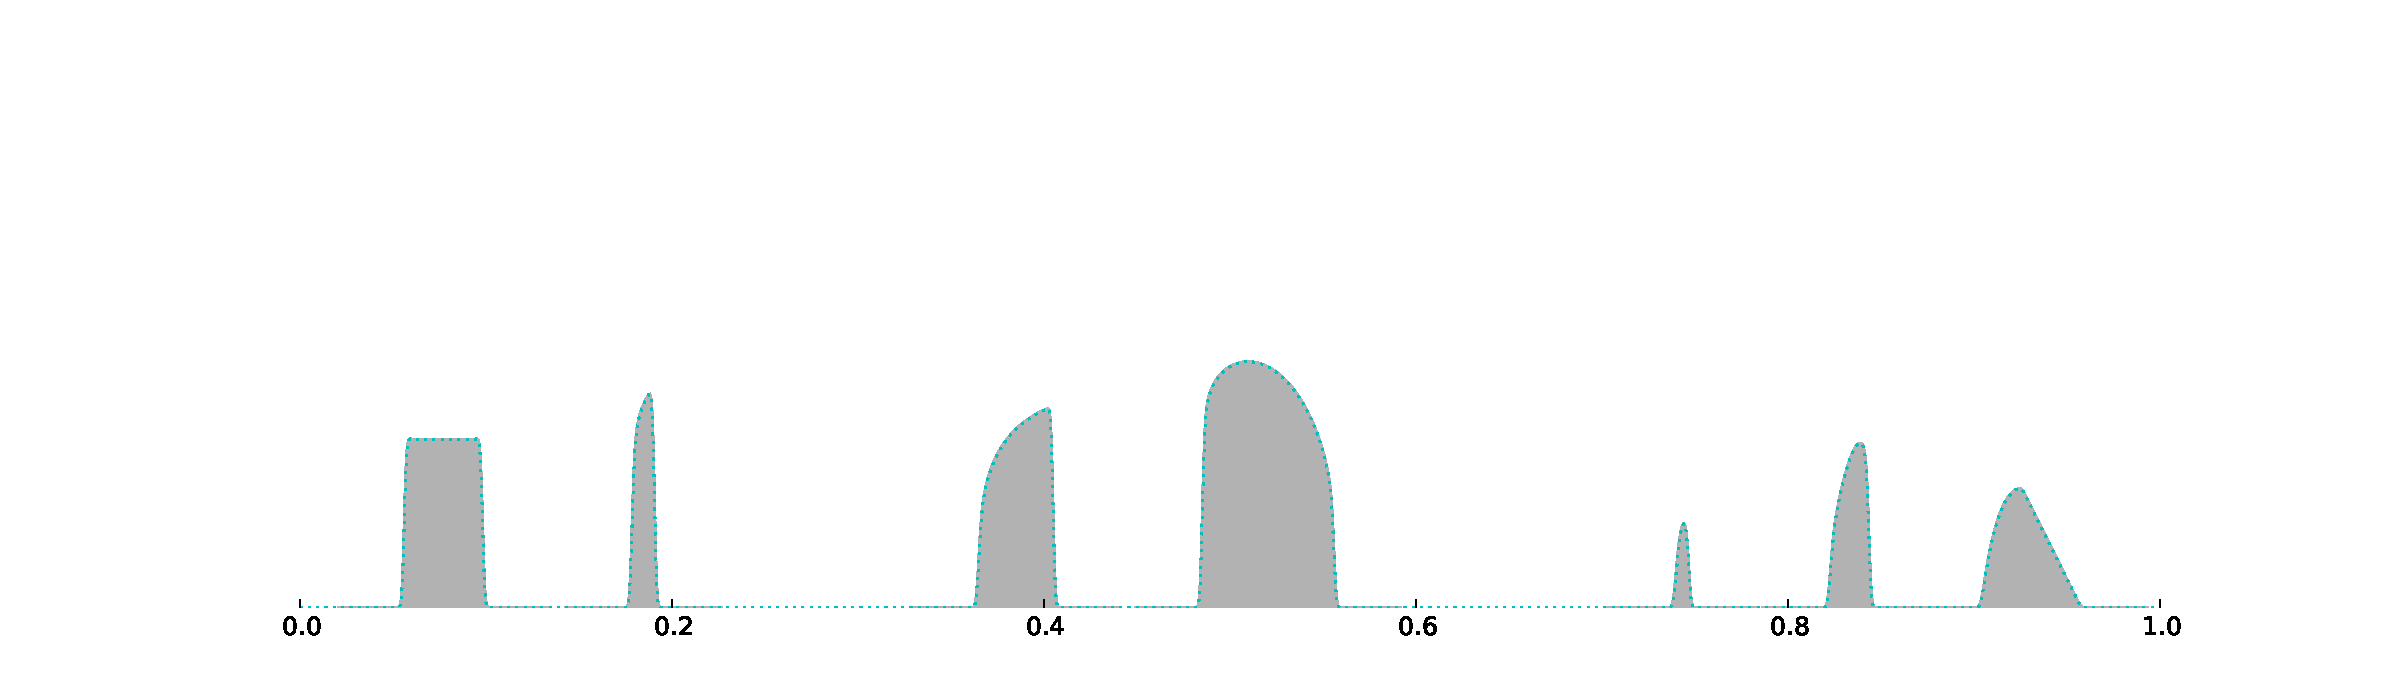
\includegraphics[clip,trim=0cm 0cm 0cm 0cm]{images/barycenter1d/barycenter1d_OT_a}
}
\caption{$\iota_{\{=\}}$}\label{fig_bary1d_OT}
\end{subfigure}
\begin{subfigure}{0.5\linewidth} 
\centering
 \resizebox{1.\linewidth}{!}{
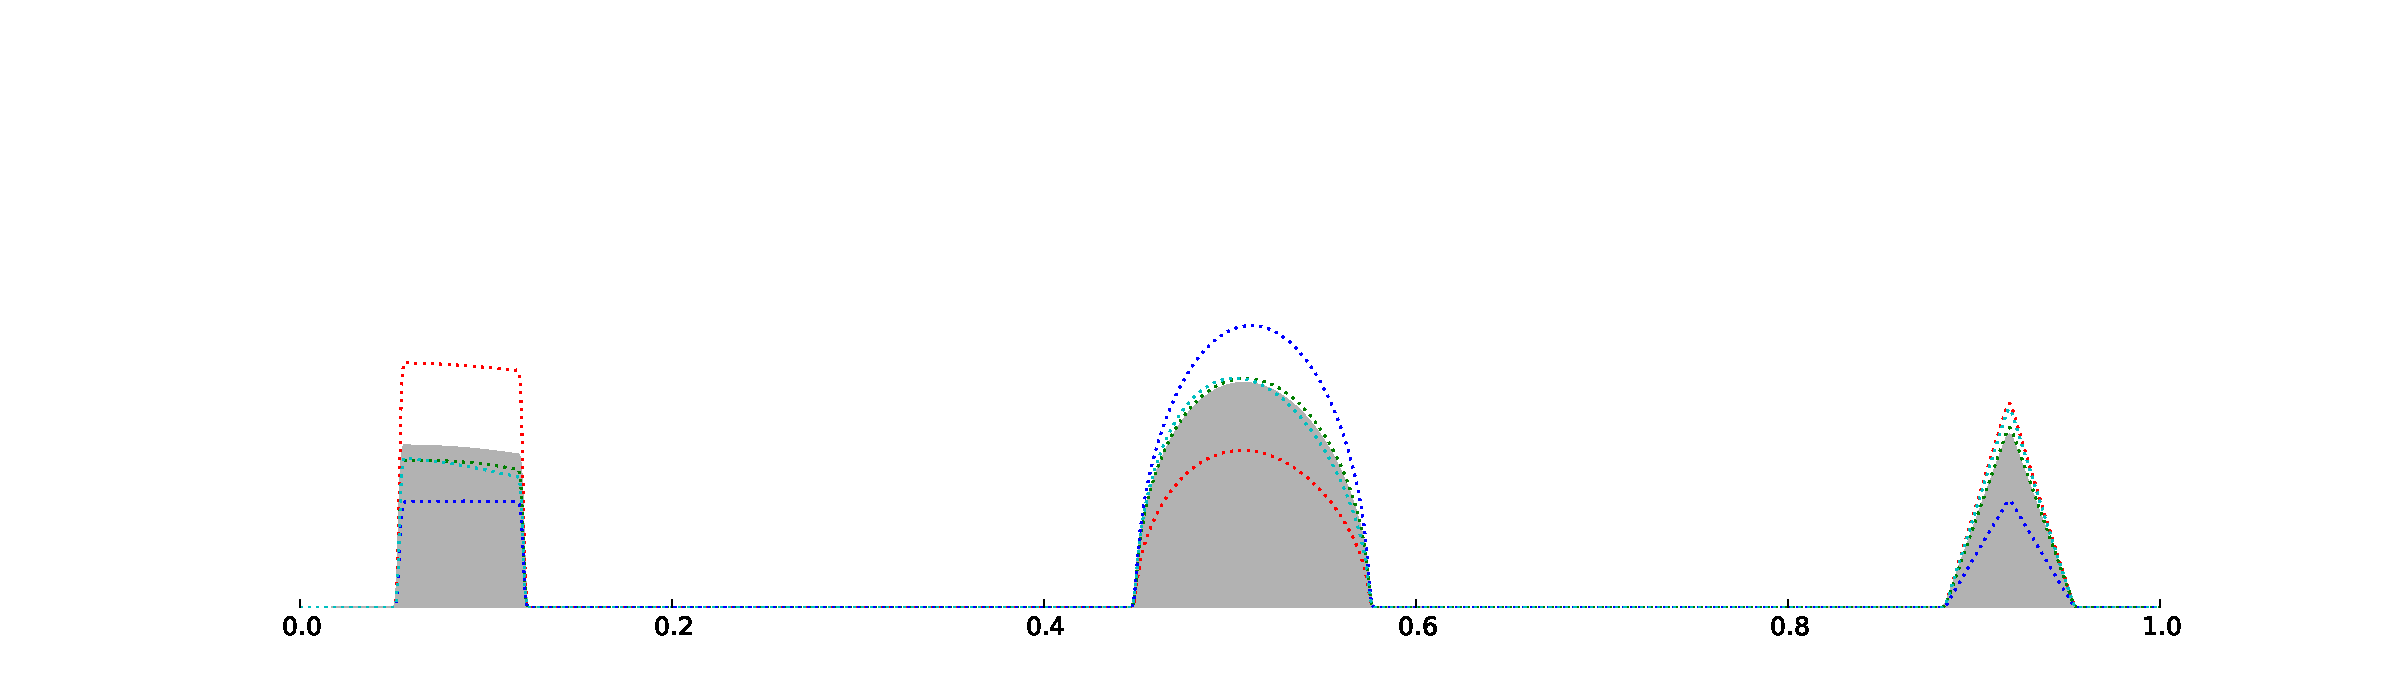
\includegraphics[clip,trim=0cm 0cm 0cm 0cm]{images/barycenter1d/barycenter1d_KL}
}
\caption{$0.07\times \KL$}\label{fig_bary1d_KL}
\end{subfigure}%
\begin{subfigure}{0.5\linewidth} 
\centering
 \resizebox{1.\linewidth}{!}{
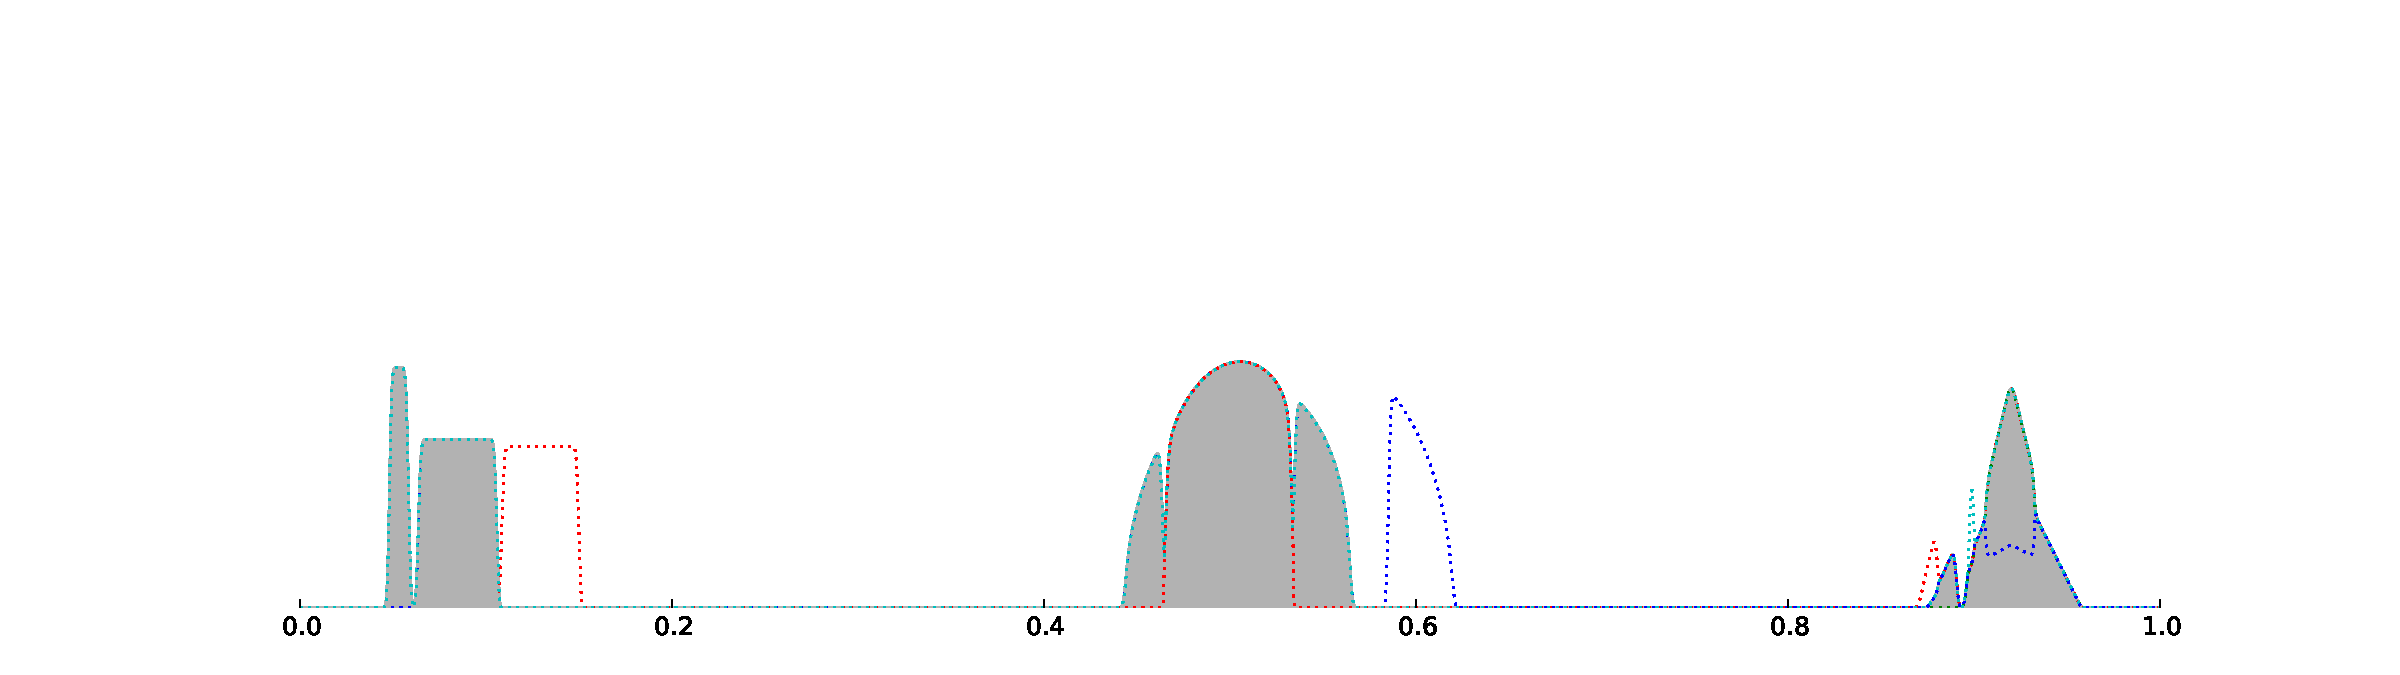
\includegraphics[clip,trim=0cm 0cm 0cm 0cm]{images/barycenter1d/barycenter1d_TV}
}
\caption{$0.02\times \TV$}
\end{subfigure}
\begin{subfigure}{0.5\linewidth} 
\centering
 \resizebox{1.\linewidth}{!}{
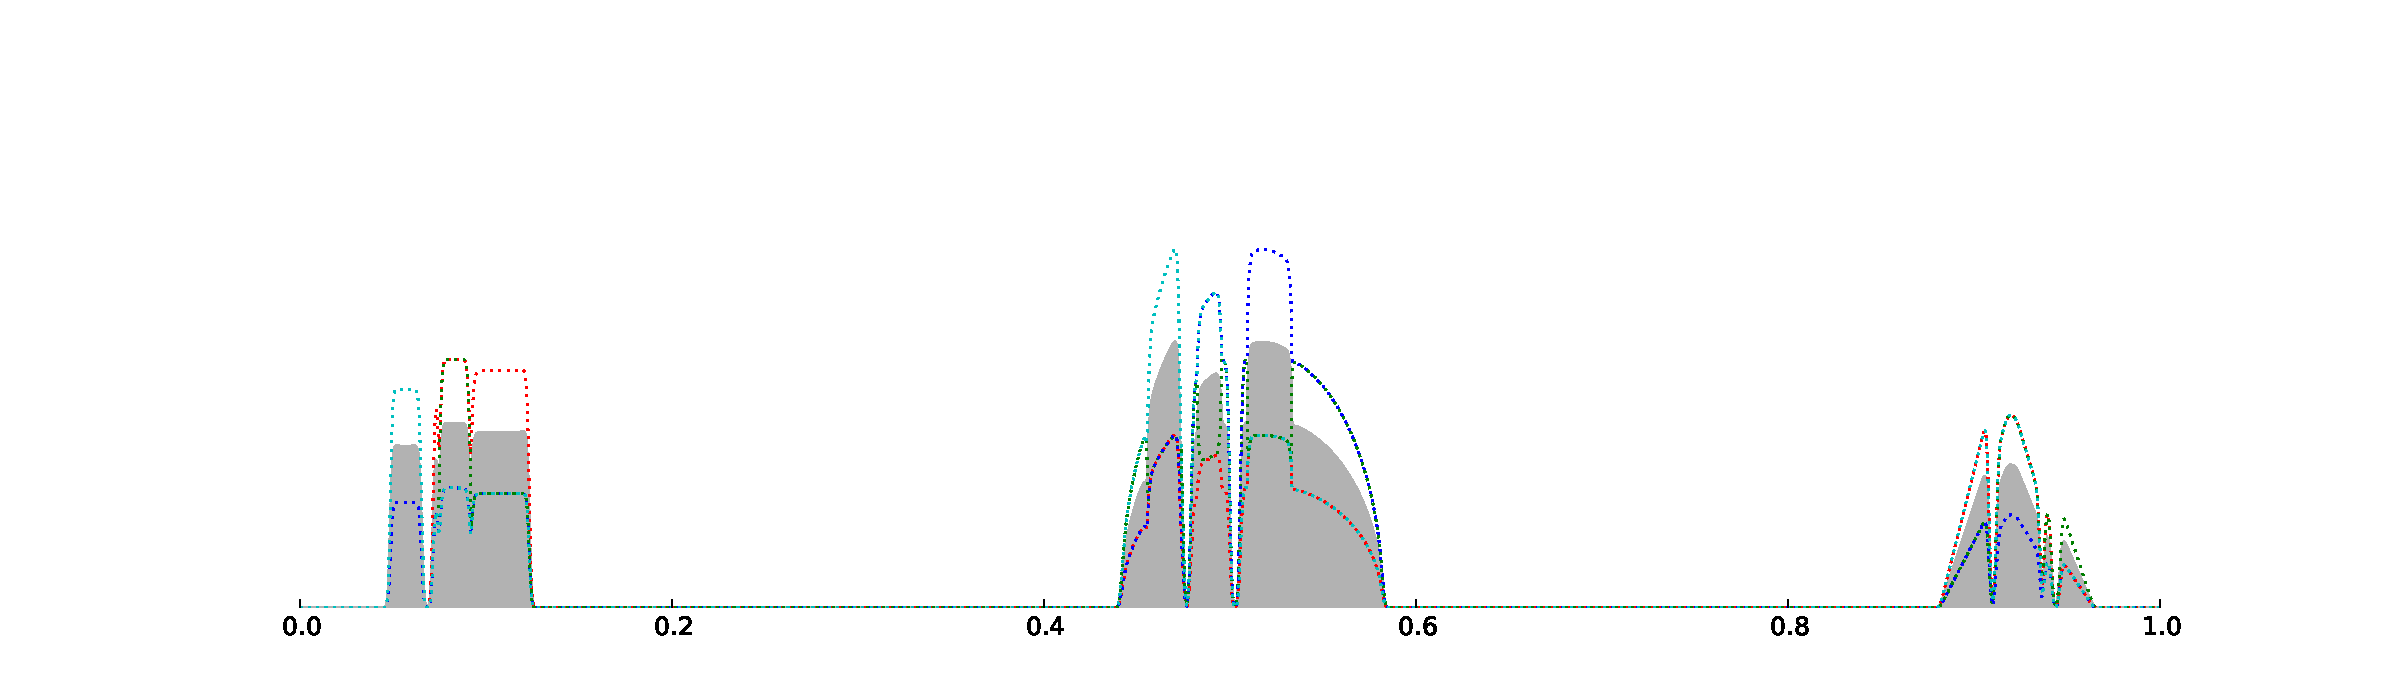
\includegraphics[clip,trim=0cm 0cm 0cm 0cm]{images/barycenter1d/barycenter1d_RG}
}
\caption{$\RG_{[0.65,\,1.35]}$}
\end{subfigure}%
\begin{subfigure}{0.5\linewidth} 
\centering
 \resizebox{1.\linewidth}{!}{
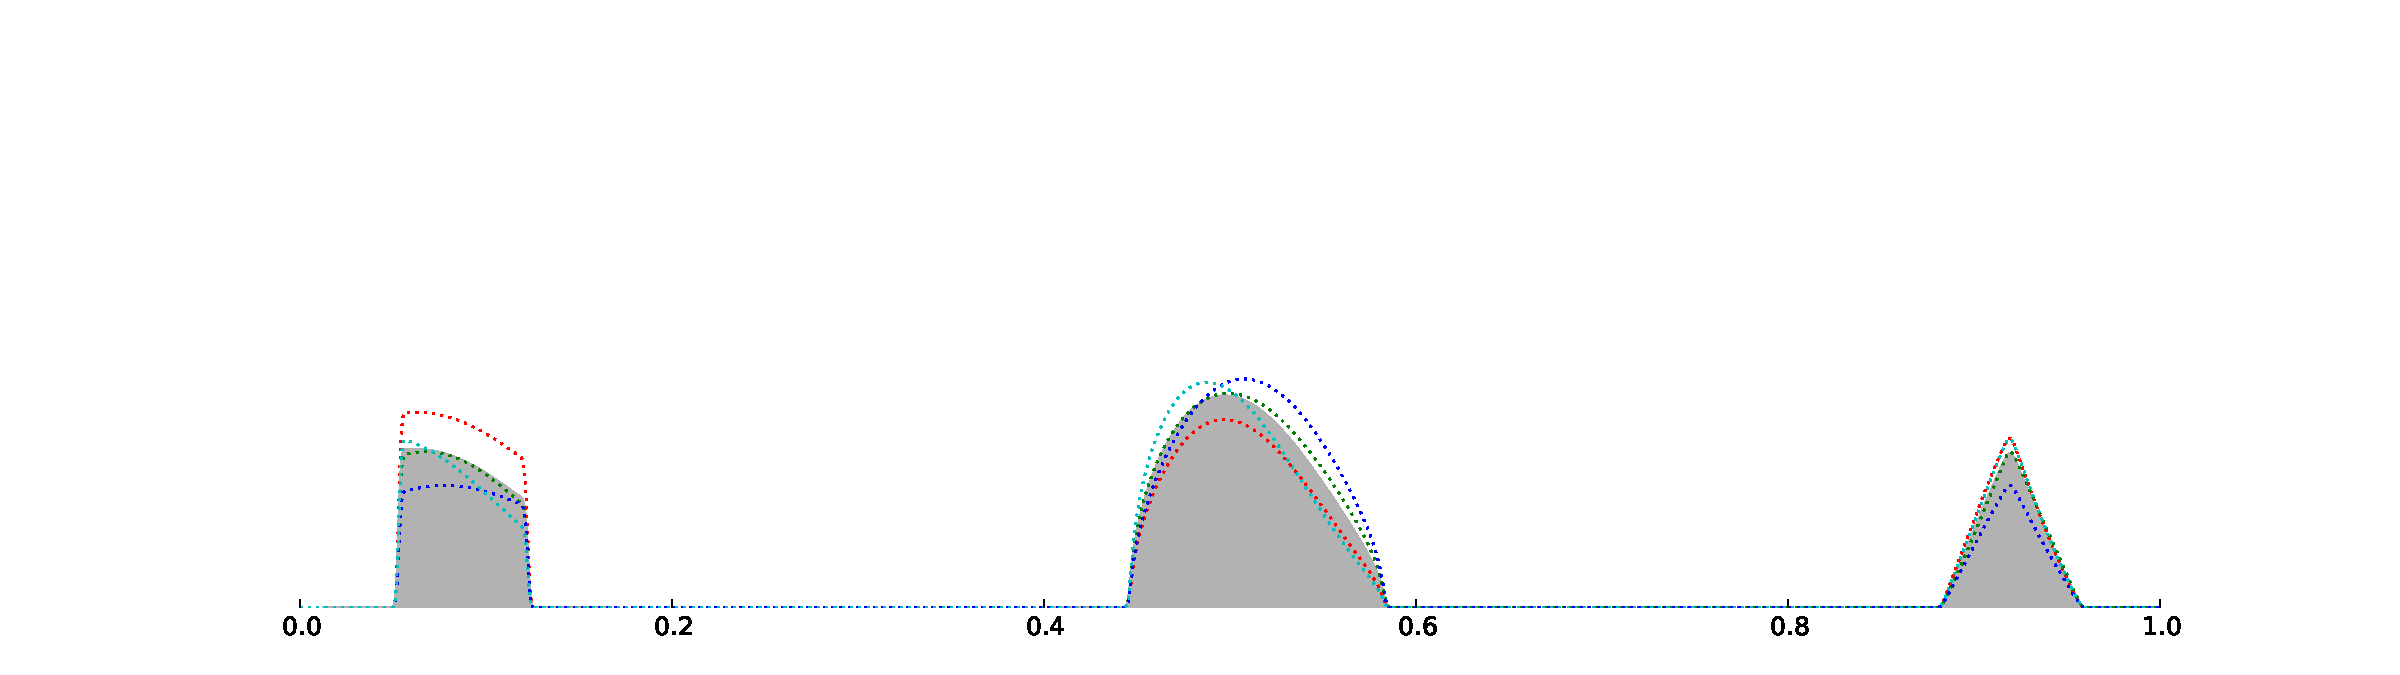
\includegraphics[clip,trim=0cm 0cm 0cm 0cm]{images/barycenter1d/barycenter1d_WF}
}
\caption{$\WF$ (cut locus at $0.2$)}\label{fig_bary1d_WF}
\end{subfigure}%
\caption{Illustration of barycenter-like problems on $X=Y=[0,1]$. Except for (f), the function $F_1$ is the equality constraint with respect to the densities $(\mathbf{p}_k)_{k=1}^4$, the cost is $c(x,y)=|y-x|^2$, the weights are $(\tfrac14,\tfrac14,\tfrac14,\tfrac14)$ and the function $F_2$ is of the type \eqref{eq_Fbary} with the divergence specified in the legend. Figure (f) represents the Fr\'echet mean for the $\WF$ metric. The dotted lines display the second marginal of the optimal plans.}
\label{fig_1Dbarycenter}
\end{figure}

%%%%%%%%%%%%%%%%%%%%%%%%%%%%%%%%%%%%%%%%%%
\pgfmathsetmacro{\ax}{33}
\pgfmathsetmacro{\ay}{25}
\pgfmathsetmacro{\b}{1.5}
%%%%%%%%%%%%%%%%%%%%%%%%%%%%%%%%%%%%%%%%%%
\begin{figure}
 \centering 
 \CompressedVersion{
 	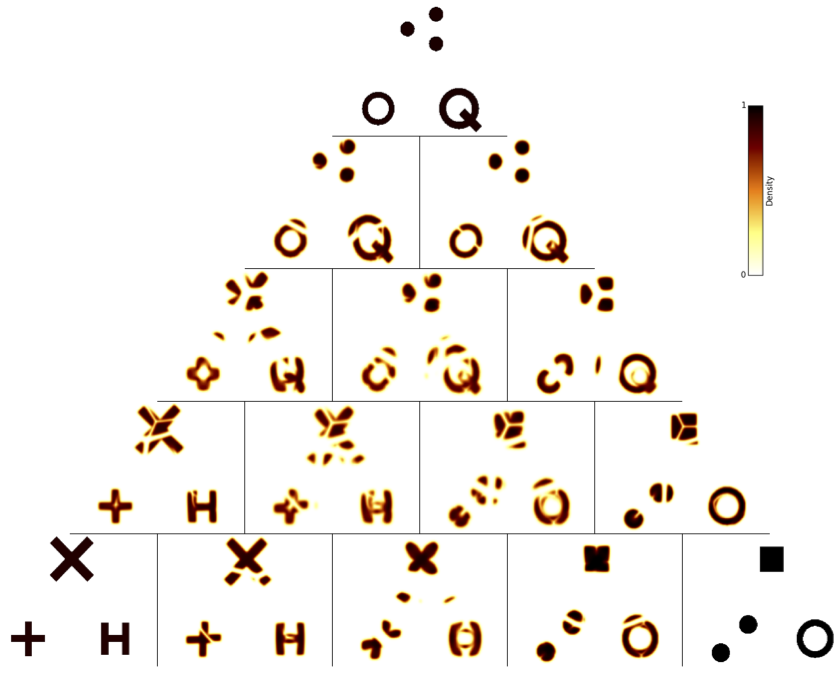
\includegraphics{images/low/bary-fig10}
 }{
  \resizebox{.9\linewidth}{!}{
\begin{tikzpicture}%y,x
\node (1) at (-\ax,-\ay) {\includegraphics[clip,trim=\b cm \b cm \b cm \b cm]{images/triangleOT2/barycenter2d_100}};
\node (2) at (0,\ay) {
\includegraphics[clip,trim=\b cm \b cm \b cm \b cm]{images/triangleOT2/barycenter2d_010}};
\node (3) at (\ax,-\ay) {\includegraphics[clip,trim=\b cm \b cm \b cm \b cm]{images/triangleOT2/barycenter2d_001}};

\node (4) at (-\ax/2,-\ay) {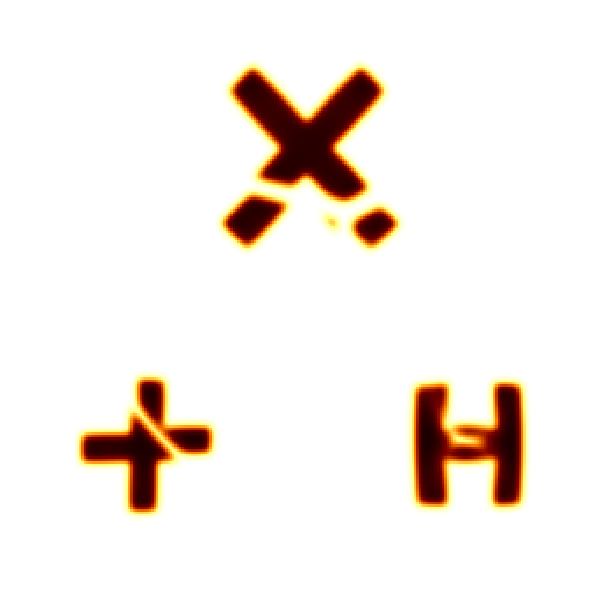
\includegraphics[clip,trim=\b cm \b cm \b cm \b cm]{images/triangleOT2/barycenter2dOT301}};
\node (5) at (0,-\ay) {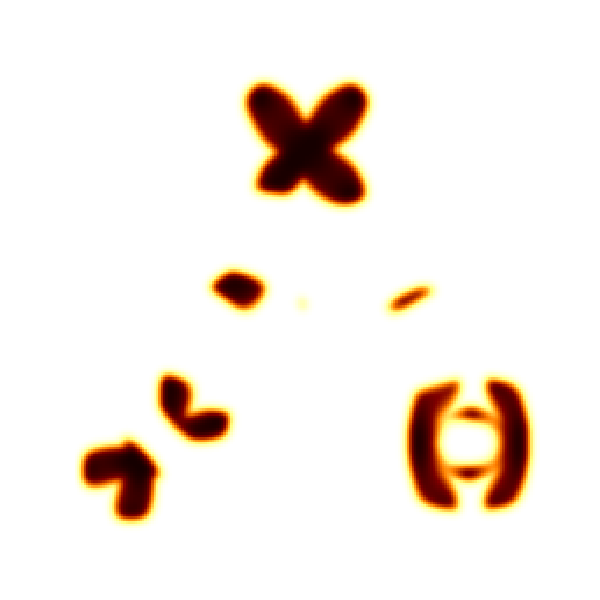
\includegraphics[clip,trim=\b cm \b cm \b cm \b cm]{images/triangleOT2/barycenter2dOT202}};
\node (6) at (\ax/2,-\ay) {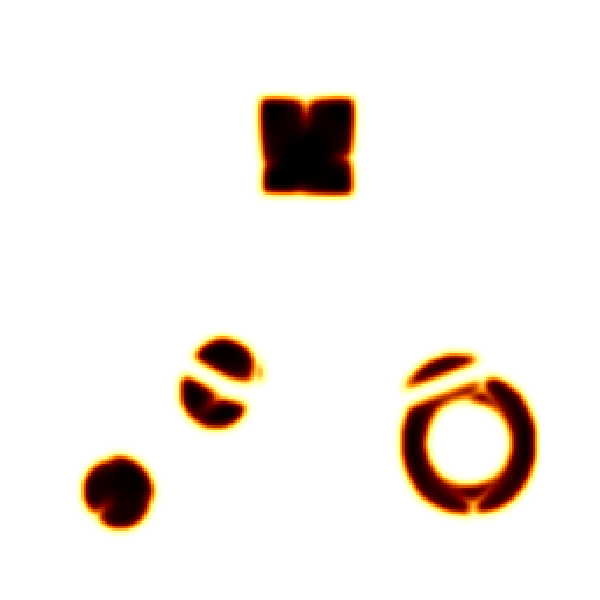
\includegraphics[clip,trim=\b cm \b cm \b cm \b cm]{images/triangleOT2/barycenter2dOT103}};

\node (7) at (-3*\ax/4,-2*\ay/4) {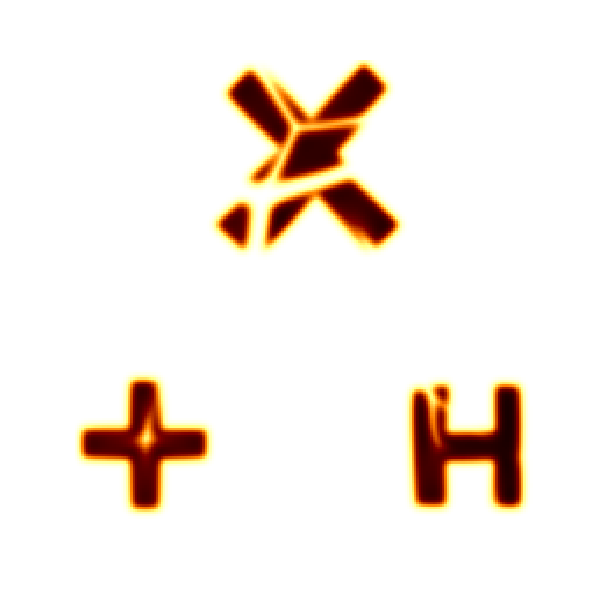
\includegraphics[clip,trim=\b cm \b cm \b cm \b cm]{images/triangleOT2/barycenter2dOT310}};
\node (8) at (-\ax/4,-2*\ay/4) {
\includegraphics[clip,trim=\b cm \b cm \b cm \b cm]{images/triangleOT2/barycenter2dOT211}};
\node (9) at (\ax/4,-2*\ay/4) {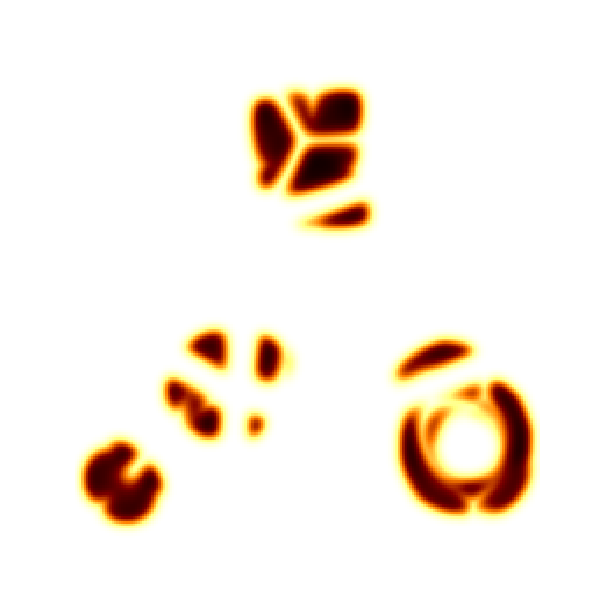
\includegraphics[clip,trim=\b cm \b cm \b cm \b cm]{images/triangleOT2/barycenter2dOT112}};
\node (10) at (3*\ax/4,-2*\ay/4) {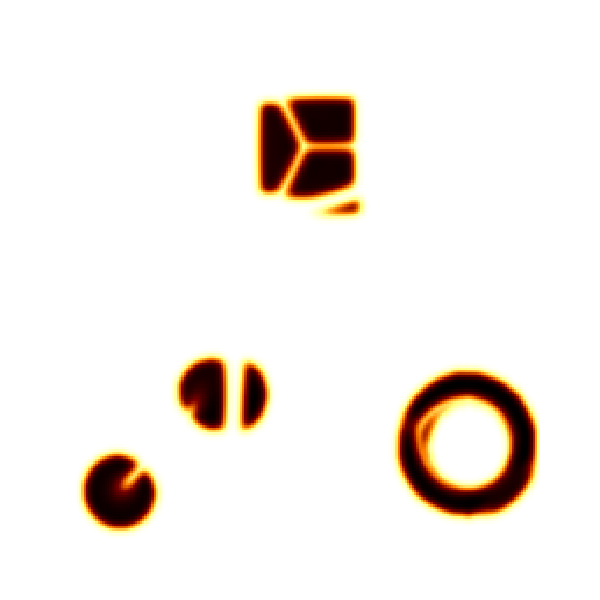
\includegraphics[clip,trim=\b cm \b cm \b cm \b cm]{images/triangleOT2/barycenter2dOT013}};

\node (11) at (-2*\ax/4,0) {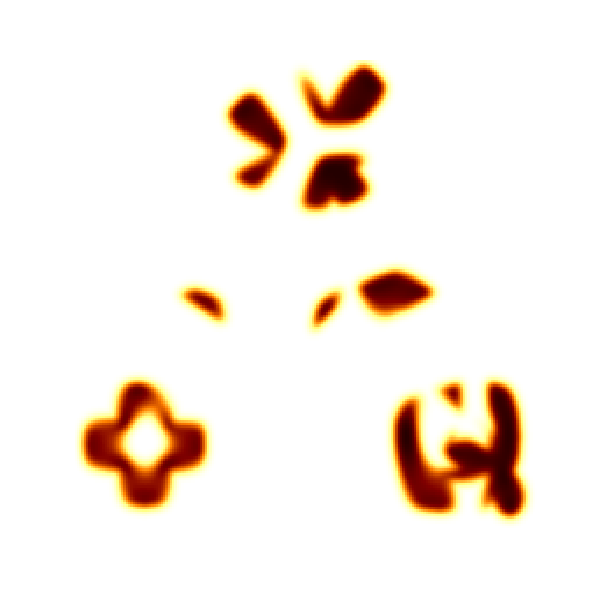
\includegraphics[clip,trim=\b cm \b cm \b cm \b cm]{images/triangleOT2/barycenter2dOT220}};
\node (12) at (0,0) {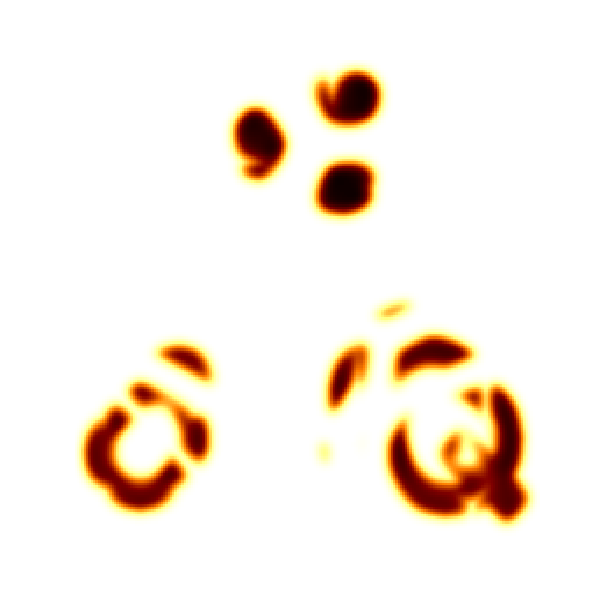
\includegraphics[clip,trim=\b cm \b cm \b cm \b cm]{images/triangleOT2/barycenter2dOT121}};
\node (13) at (2*\ax/4,0) {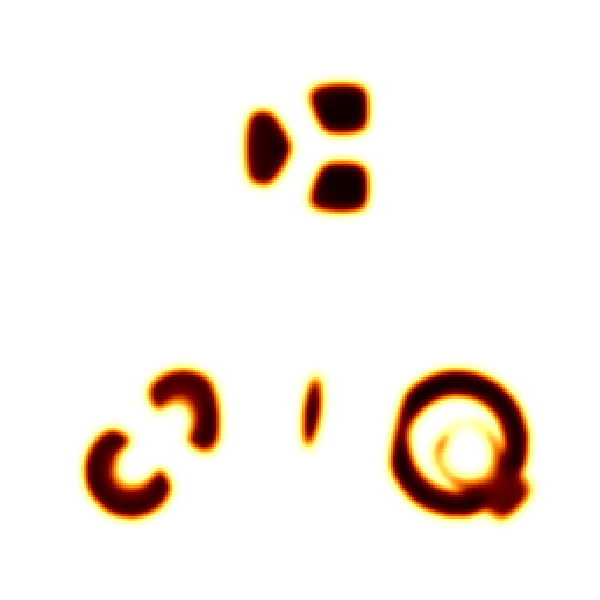
\includegraphics[clip,trim=\b cm \b cm \b cm \b cm]{images/triangleOT2/barycenter2dOT022}};

\node (14) at (-\ax/4,\ay/2) {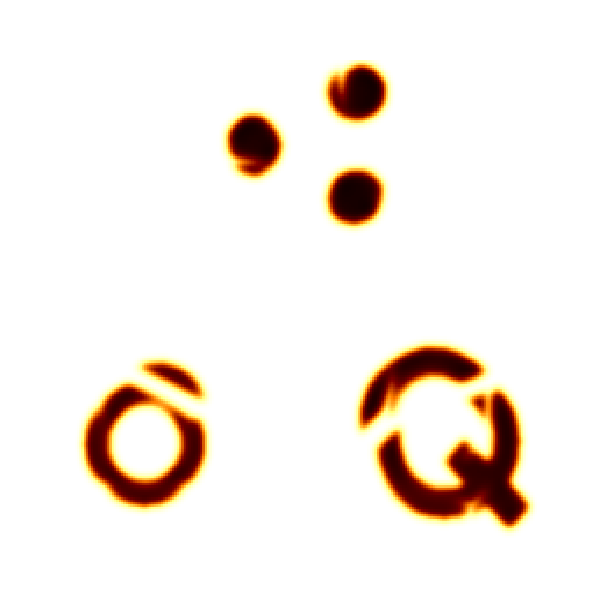
\includegraphics[clip,trim=\b cm \b cm \b cm \b cm]{images/triangleOT2/barycenter2dOT130}};
\node (15) at (\ax/4,\ay/2) {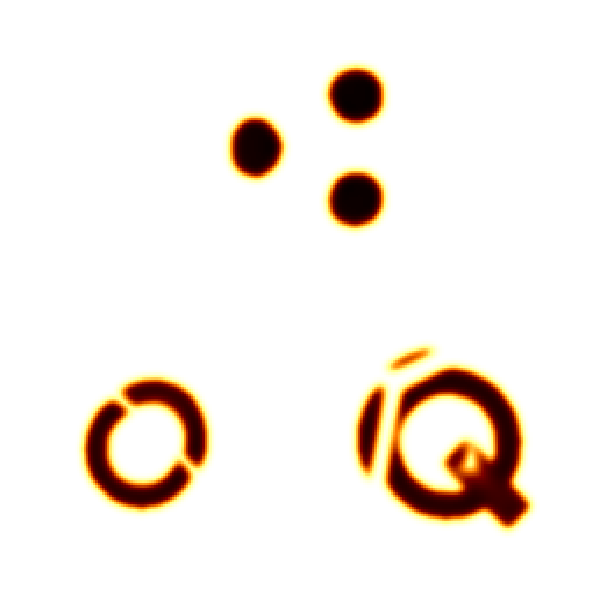
\includegraphics[clip,trim=\b cm \b cm \b cm \b cm]{images/triangleOT2/barycenter2dOT031}};

\node (15) at (\ax,\ay/2) {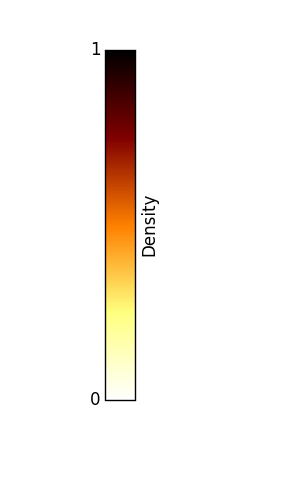
\includegraphics[scale=1.8]{images/triangleKL2/cmapbary}};

\draw[thick] 	(-\ax/4,3*\ay/4)    	-- 	(\ax/4,3*\ay/4);
\draw[thick] 	(-2*\ax/4,\ay/4)    	-- 	(2*\ax/4,\ay/4);
\draw[thick] 	(-3*\ax/4,-\ay/4)    	-- 	(3*\ax/4,-\ay/4);
\draw[thick] 	(-4*\ax/4,-3*\ay/4)    	-- 	(4*\ax/4,-3*\ay/4);

\draw[thick] 	(0,3*\ay/4)    	-- 	(0,1*\ay/4);
\draw[thick] 	(-\ax/4,1*\ay/4)    	-- 	(-\ax/4,-1*\ay/4);
\draw[thick] 	(\ax/4,1*\ay/4)    	-- 	(\ax/4,-1*\ay/4);
\draw[thick] 	(0,-\ay/4)    	-- 	(0,-3*\ay/4);
\draw[thick] 	(-\ax/2,-\ay/4)    	-- 	(-\ax/2,-3*\ay/4);
\draw[thick] 	(\ax/2,-\ay/4)    	-- 	(\ax/2,-3*\ay/4);
\draw[thick] 	(-\ax/4,-3*\ay/4)    	-- 	(-\ax/4,-5*\ay/4);
\draw[thick] 	(\ax/4,-3*\ay/4)    	-- 	(\ax/4,-5*\ay/4);
\draw[thick] 	(-3*\ax/4,-3*\ay/4)    	-- 	(-3*\ax/4,-5*\ay/4);
\draw[thick] 	(3*\ax/4,-3*\ay/4)    	-- 	(3*\ax/4,-5*\ay/4);
%\draw[dotted]        (2,0) -- (10,0);

\end{tikzpicture}
        }
        }
\caption{Wasserstein barycenters with entropic smoothing}
\label{fig_wasserstein_triangle}
\end{figure}

%%%%%%%%%%%%%%%%%%%%%%%%%%%%%%%%%%%%%%%%%%
\begin{figure}
 \centering
  \CompressedVersion{
 	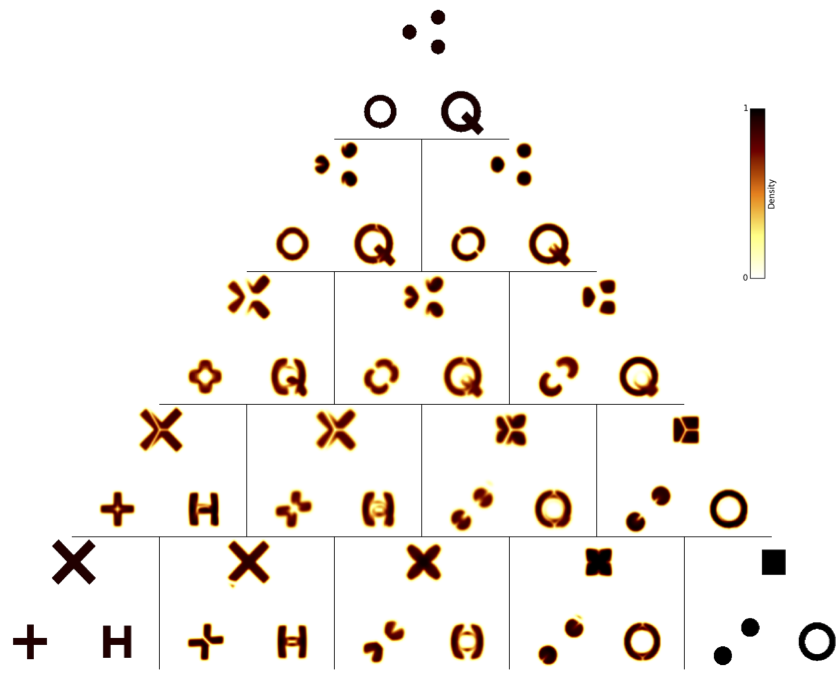
\includegraphics{images/low/bary-fig11}
 }{
  \resizebox{.9\linewidth}{!}{
\begin{tikzpicture}%y,x
\node (1) at (-\ax,-\ay) {\includegraphics[clip,trim=\b cm \b cm \b cm \b cm]{images/triangleKL2/barycenter2d_100}};
\node (2) at (0,\ay) {
\includegraphics[clip,trim=\b cm \b cm \b cm \b cm]{images/triangleKL2/barycenter2d_010}};
\node (3) at (\ax,-\ay) {\includegraphics[clip,trim=\b cm \b cm \b cm \b cm]{images/triangleKL2/barycenter2d_001}};

\node (4) at (-\ax/2,-\ay) {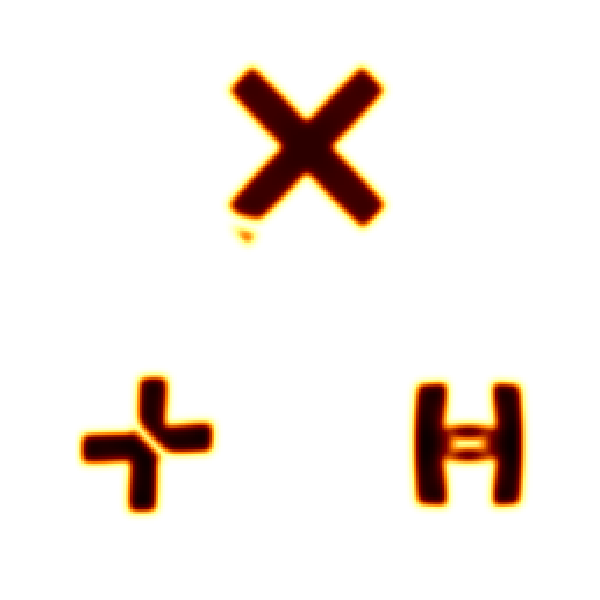
\includegraphics[clip,trim=\b cm \b cm \b cm \b cm]{images/triangleKL2/barycenter2dKL301}};
\node (5) at (0,-\ay) {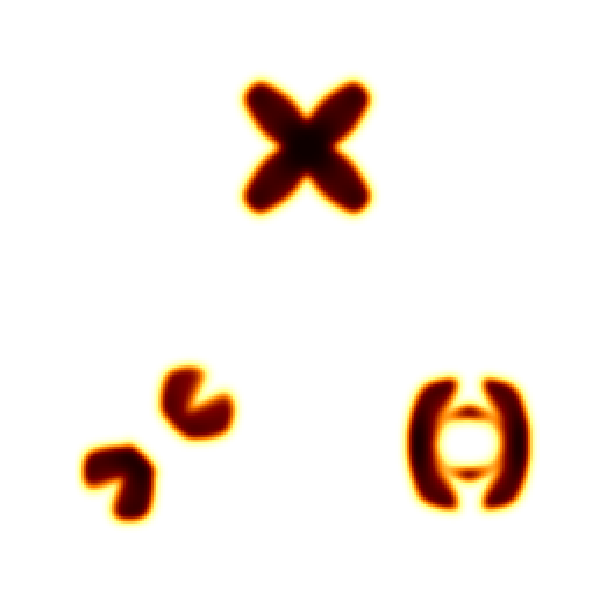
\includegraphics[clip,trim=\b cm \b cm \b cm \b cm]{images/triangleKL2/barycenter2dKL202}};
\node (6) at (\ax/2,-\ay) {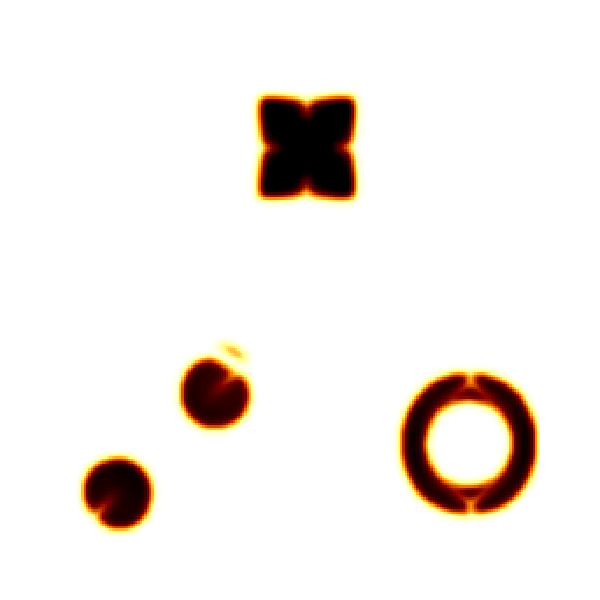
\includegraphics[clip,trim=\b cm \b cm \b cm \b cm]{images/triangleKL2/barycenter2dKL103}};

\node (7) at (-3*\ax/4,-2*\ay/4) {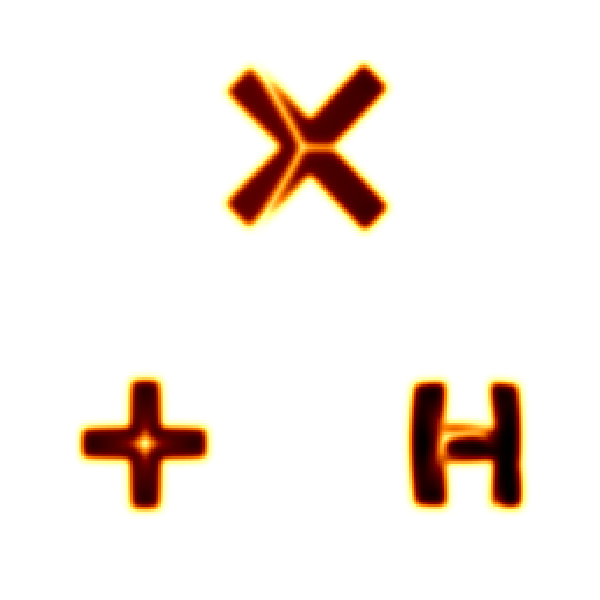
\includegraphics[clip,trim=\b cm \b cm \b cm \b cm]{images/triangleKL2/barycenter2dKL310}};
\node (8) at (-\ax/4,-2*\ay/4) {
\includegraphics[clip,trim=\b cm \b cm \b cm \b cm]{images/triangleKL2/barycenter2dKL211}};
\node (9) at (\ax/4,-2*\ay/4) {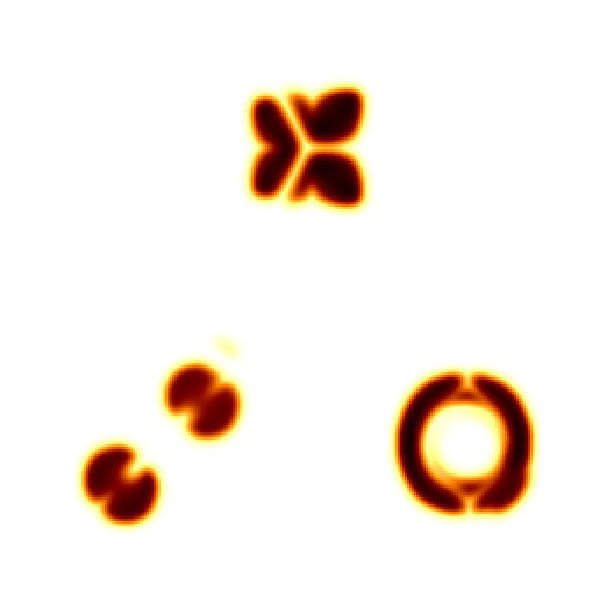
\includegraphics[clip,trim=\b cm \b cm \b cm \b cm]{images/triangleKL2/barycenter2dKL112}};
\node (10) at (3*\ax/4,-2*\ay/4) {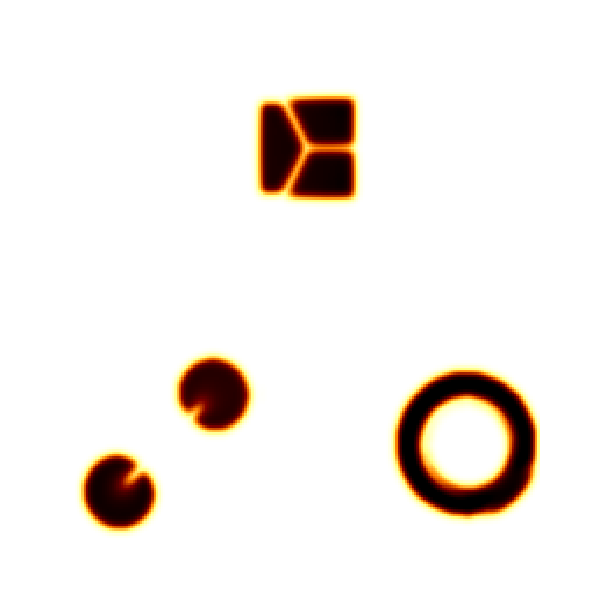
\includegraphics[clip,trim=\b cm \b cm \b cm \b cm]{images/triangleKL2/barycenter2dKL013}};

\node (11) at (-2*\ax/4,0) {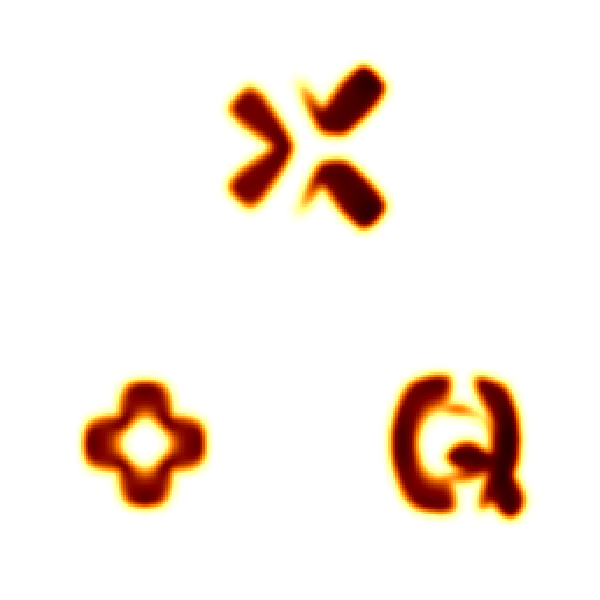
\includegraphics[clip,trim=\b cm \b cm \b cm \b cm]{images/triangleKL2/barycenter2dKL220}};
\node (12) at (0,0) {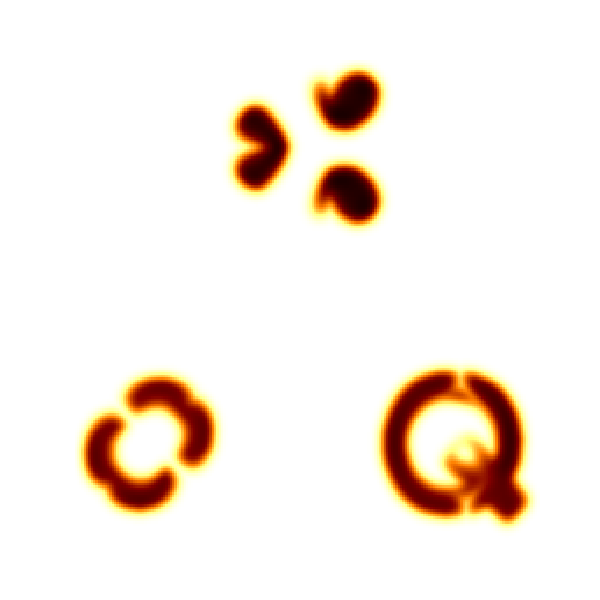
\includegraphics[clip,trim=\b cm \b cm \b cm \b cm]{images/triangleKL2/barycenter2dKL121}};
\node (13) at (2*\ax/4,0) {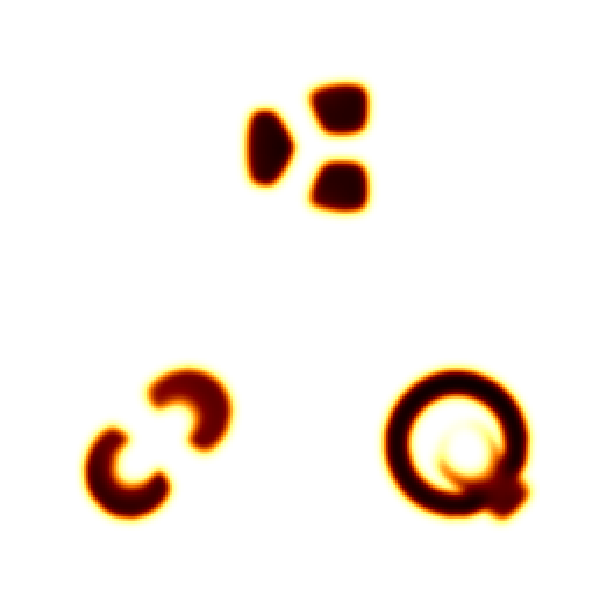
\includegraphics[clip,trim=\b cm \b cm \b cm \b cm]{images/triangleKL2/barycenter2dKL022}};

\node (14) at (-\ax/4,\ay/2) {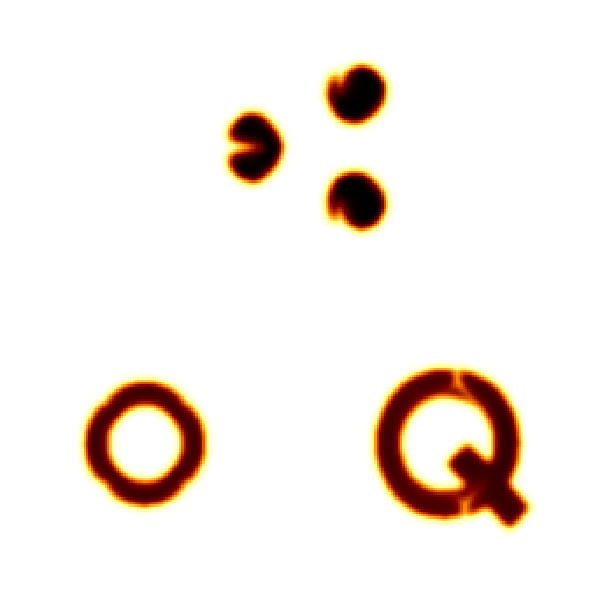
\includegraphics[clip,trim=\b cm \b cm \b cm \b cm]{images/triangleKL2/barycenter2dKL130}};
\node (15) at (\ax/4,\ay/2) {
\includegraphics[clip,trim=\b cm \b cm \b cm \b cm]{images/triangleKL2/barycenter2dKL031}};

\node (15) at (\ax,\ay/2) {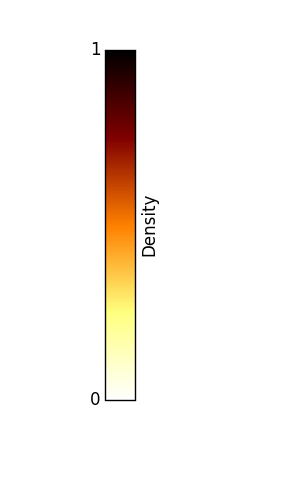
\includegraphics[scale=1.8]{images/triangleKL2/cmapbary}};

\draw[thick] 	(-\ax/4,3*\ay/4)    	-- 	(\ax/4,3*\ay/4);
\draw[thick] 	(-2*\ax/4,\ay/4)    	-- 	(2*\ax/4,\ay/4);
\draw[thick] 	(-3*\ax/4,-\ay/4)    	-- 	(3*\ax/4,-\ay/4);
\draw[thick] 	(-4*\ax/4,-3*\ay/4)    	-- 	(4*\ax/4,-3*\ay/4);

\draw[thick] 	(0,3*\ay/4)    	-- 	(0,1*\ay/4);
\draw[thick] 	(-\ax/4,1*\ay/4)    	-- 	(-\ax/4,-1*\ay/4);
\draw[thick] 	(\ax/4,1*\ay/4)    	-- 	(\ax/4,-1*\ay/4);
\draw[thick] 	(0,-\ay/4)    	-- 	(0,-3*\ay/4);
\draw[thick] 	(-\ax/2,-\ay/4)    	-- 	(-\ax/2,-3*\ay/4);
\draw[thick] 	(\ax/2,-\ay/4)    	-- 	(\ax/2,-3*\ay/4);
\draw[thick] 	(-\ax/4,-3*\ay/4)    	-- 	(-\ax/4,-5*\ay/4);
\draw[thick] 	(\ax/4,-3*\ay/4)    	-- 	(\ax/4,-5*\ay/4);
\draw[thick] 	(-3*\ax/4,-3*\ay/4)    	-- 	(-3*\ax/4,-5*\ay/4);
\draw[thick] 	(3*\ax/4,-3*\ay/4)    	-- 	(3*\ax/4,-5*\ay/4);
\end{tikzpicture}
        }
       }
\caption{$\GHK$ barycenters with entropic smoothing (the definition of the $\GHK$ metric is similar to Wasserstein but the marginal constraints are replaced by $\KL$ divergences, see Section  \ref{subsec_unbalanced}).}
\label{fig_GHK_triangle}
\end{figure}
%%%%%%%%%%%%%%%%%%%%%%%%%%%%%%%%%%%%%%%%%%